\chapter{Trial Wave Function}
\label{ch:trial}
An accurate trial wave function can drastically improve the accuracy of QMC methods such as VMC and AFDMC by lowering the variance and improving the fermion constraint. Most highly accurate trial wave functions are computationally intractable and are never implemented in QMC methods. In addition to being accurate and computationally tractable a good wave function must satisfy known physical properties such as cluster decomposition as well as having an overall antisymmetry with respect to particle exchange due to the spin-1/2 property of nucleons.

Cluster decomposition arises from the physical intuition that the wave function of two separate, non-interacting systems, $A$ and $B$ as in Figure~\ref{fig:cluster}, can be written as the outer product of their respective wave functions $\ket{A+B}=\ket{A}\ket{B}$.
\begin{figure}[h]
   \centering
   \begin{tikzpicture}[>=latex,scale=0.5]
      \shade[ball color=blue!10!] (-4.0,0.85) circle (1) ;
      \shade[ball color=blue!10!] (-2.5,-0.85) circle (1) ;
      \shade[ball color=blue!10!] (4.0,1.35) circle (1) ;
      \shade[ball color=blue!10!] (2.5,0.00) circle (1) ;
      \draw (-3.5,-2.5) node{\large $\ket{A}$};
      \draw (3.5,-1.5) node{\large $\ket{B}$};
   \end{tikzpicture}
   \caption{Two non interacting systems $A$ and $B$, whose composite wave function is the product $\ket{A+B}=\ket{A}\ket{B}$.}
   \label{fig:cluster}
\end{figure}
If a system is not cluster decomposable, nonphysical correlations between non-interacting systems can occur. I will now define a strong and weak condition on cluster decomposability. There exist systems that are cluster decomposable, in that they obey the description above, yet they lack all of the proper correlations between particles in the respective systems. This will be referred to as the weak condition of cluster decomposition. Many of the approximate wave functions that I will describe later will obey only this weak condition. It is important to note that the weak condition does not contain any unphysical correlations, they simply lack some or all of the physical correlations of the system. The strong condition of cluster decomposition is that the above condition is obeyed and each subsystem contains all of the appropriate correlations for that system. This will be illuminated when our specific wave functions are described.

The second property is that the wave function be antisymmetric overall. Since nucleons are fermions and the only degrees of freedom used in these calculations the product of different pieces of the wave function must be antisymmetric. Recent work in QMC has successfully included bosonic degrees of freedom such as pions (\cite{madeira2018}), however that is not the case in this work.

%\begin{figure}[h!]
%   \centering
%   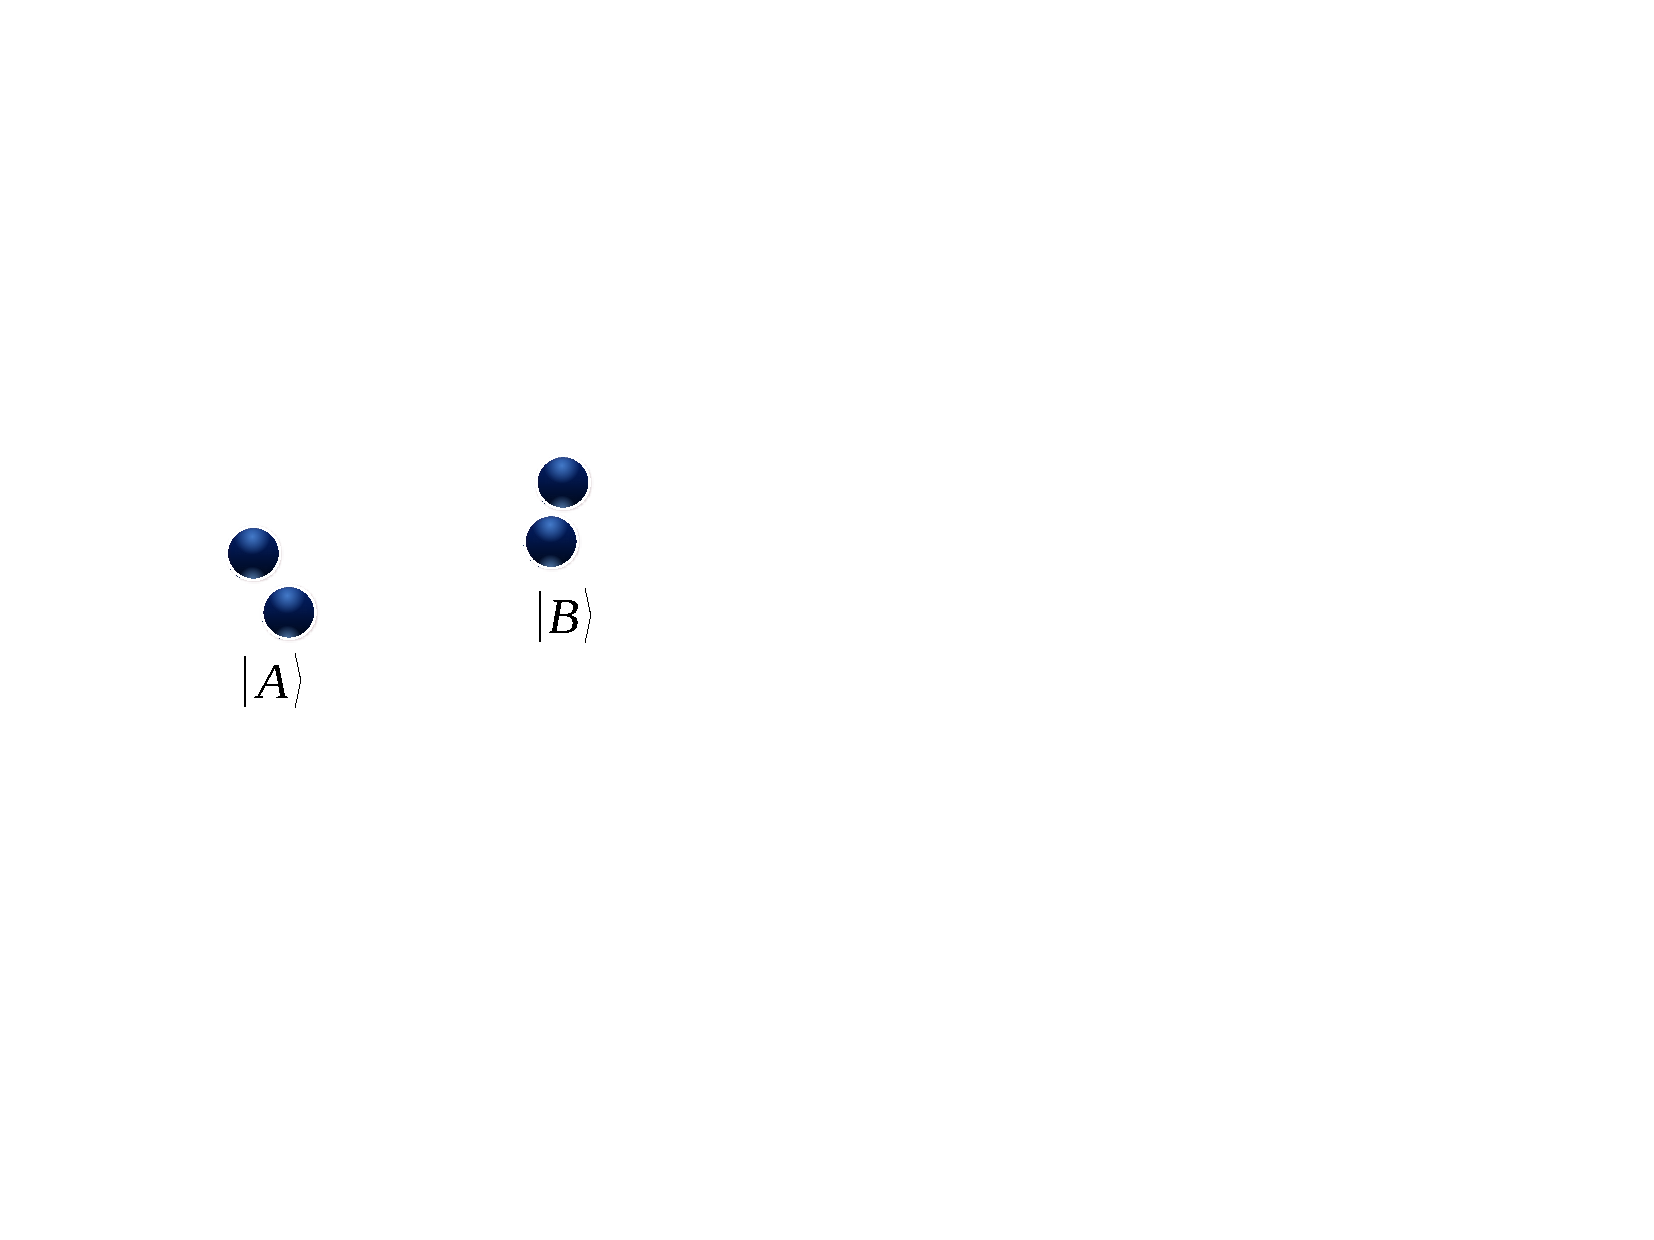
\includegraphics[width=\textwidth]{figures/cluster.pdf}
%   \caption{Energy per nucleon for ${}^4$He and ${}^{16}$O as calculated with linear, independent pair and quadratic correlations. Also, the energy per nucleon of symmetric nuclear matter of 28 particles in a periodic box with density $\rho=0.16$fm$^{-3}$. All calculations are compared to their expected values.}
%   \label{fig:cluster}
%\end{figure}

\section{Slater Determinant}
As used in this work one of the simplest wave functions that satisfies the two properties specified above is the Slater determinant. The Slater determinant has been the starting place for a variety of many-body calculations in nuclear and condensed matter physics alike. In electronic calculations the many-body wave functions will often be written in terms of a sum of weighted Slater determinants, where some methods have been able to use a sum of up to 2 billion determinants for the semistochastic heat-bath configuration interaction method (\cite{huron1973,li2018}). The no-core shell-model, used in nuclear physics, also uses a sum of Slater determinants (\cite{navratil2009,barrett2013}), often written in a truncated harmonic oscillator basis, where the number of determinants is based on the maximally allowed harmonic oscillator energy for the $A$ nucleon system. In QMC calculations a single, or sum of Slater determinants is often also used, however the single particle states are written to have good spin, isospin, and angular momentum quantum numbers. A single determinant is often used as a model state for closed shell calculations and a sum of small number of weighted determinants is used for open shell systems, to maintain good quantum numbers for the system. For small to medium mass open-shell nuclei on the order of 10 or 100 determinants are often used for a model state. A Slater determinant is an antisymmetrized product of single particle, non-interacting, wave functions
\begin{equation}
   \Psi_{SD}(\R) = \mathcal{A} \left[\phi_1(\r_1)\phi_2(\r_2) \ldots \phi_A(\r_A)\right] =
   \begin{vmatrix}
      \phi_1(\r_1) & \phi_1(\r_2) & \ldots & \phi_1(\r_A) \\
      \phi_2(\r_1) & \phi_2(\r_2) & \ldots & \phi_2(\r_A) \\
      \vdots & \vdots & \ddots & \vdots \\
      \phi_K(\r_1) & \phi_K(\r_2) & \ldots & \phi_K(\r_A) \\
   \end{vmatrix},
\end{equation}
where $\R$ contains the spatial and spin-isospin coordinates of the walkers, $\mathcal{A}$ is the antisymmetrization operator, and the $\phi_i(\r_j)$ are the overlap of the walker positions with the model single particle states, $\braket{\r_j}{\phi_i}$. The $\r_i$ coordinates are relative to the center of mass $\r_i = \mathbf{u}_i - \frac{1}{A}\sum_jm_j\mathbf{u}_j$, where $\mathbf{u}_i$ are the nucleon coordinates relative to some origin. The single particle model states are made up of a radial and spin, iso-spin dependent parts,
\begin{equation}
   \phi_k = \Phi_{nj}\left[C_{c_l,m_s}^j Y_{l,m_l}(\hat{r}_i)\chi_s(s_i)\right]_{j,m_j},
\end{equation}
where $\Phi_{nj}$ is the radial part and the rest contains the spherical harmonics $Y_{l,m_l}(\hat{r}_I)$ and spin and iso-spin states where the Clebsch-Gordan coefficients ensure the correct $j$ and $m_j$ quantum numbers, and the different states are given by the index $k$. To accurately describe the wave function of an open shell nuclei each state with the correct total angular momentum, parity $J^\pi$, and isospin $T$ is included as a separate Slater determinant.
\begin{equation}
   \braket{\R S}{\Phi}_{J^\pi,T} = \sum\limits_n c_n D\{\phi_k(\r_i,s_i)\}
\end{equation}
Here the $c_n$ coefficients are variational parameters used to minimize the energy given a set of possible state configurations. One of the simplest examples of an open shell nuclei would be $^6$He whose ground state is a $J^\pi = 0^+$ state. The two protons and two of the neutrons could be in the full $(1S_{1/2})^2$ shell while the two remaining neutrons could be in the $(1P_{3/2})^2$ shell with their $m_j=\pm 3/2, \pm 1/2$ values being equal and opposite to ensure that $J=0$. This state has two possible determinants. Other possible configurations for the two remaining neutrons would be $(1P_{1/2})^2$ with one possible determinant, $(1D_{5/2})^2$ with three possible determinants, $(2S_{1/2})^2$ with one possible determinant and $(1D_{3/2})^2$ with two possible determinants giving a total of nine possible determinants. Notice that the two neutrons could be in a combination of $S$ and $D$ shells but never an $S$ and $P$ or $D$ and $P$ to ensure the parity of the state is positive. The number of determinants used for the model states of open shell nuclei will control how accurate the trial wave function is. For closed shell nuclei such as $^4$He or $^{16}$O a single Slater determinant describing the full shell configuration is sufficient.

In the calculations described here, the radial part $\Phi_{nj}$ of the single particle states are obtained as bound state solutions to the single particle Schr\"odinger equation with a Woods-Saxon potential wine-bottle potential.
\begin{equation}
   v(r) = V_s\left[\frac{1}{1+e^{(r-r_s)/a_s}} + \alpha_se^{(-r/\rho_s)^2}\right]
\end{equation}
Here the parameters, $V_s, r_s, a_s, \alpha_s$ and $\rho_s$ are variational parameters used to shape the potential to obtain a minimum in energy.

%As an illustrative example consider the deuteron. The deuteron is in a iso-spin singlet state, $\frac{1}{\sqrt{2\pi}}(\ket{pn}-\ket{np})$. To show how the model state, $\ket{\Phi}$ would be built for this I will assume all entries are 1, though in practice the could all take on different numbers to account for the different spacial and spin dependencies of the state. Let's assume that both the neutron and the proton are in a spin up state. In this case the $\Phi(k,i)$ terms, where $k,i=1,2$, would take on the following values.
%\begin{align}
%   \phi(1,1)&=(1,0,0,0)=p\uparrow_1 \\
%   \phi(2,1)&=(0,0,1,0)=n\uparrow_1 \\
%   \phi(1,2)&=(1,0,0,0)=p\uparrow_2 \\
%   \phi(2,2)&=(0,0,1,0)=n\uparrow_2
%\end{align}
%The determinant of the Slater matrix can then be written as
%\begin{equation}
%\Psi_T=\det(S)=
%\begin{vmatrix}
%    \braket{k_1}{s_1} & \braket{k_1}{s_2} \\
%    \braket{k_2}{s_1} & \braket{k_2}{s_2}
%\end{vmatrix}
%=
%\begin{vmatrix}
%    p_1 & p_2 \\
%    n_1 & n_2
%\end{vmatrix}
%=
%p_1n_2-n_1p_2,
%\end{equation}
%which is the singlet state that we wanted to start with.

The Slater determinant is a mean-field wave function and is often used with Jastrow type short range correlations.
\begin{equation}
   \braket{\R S}{\psi_T} = \bra{\R S}\prod\limits_{i<j}f(r_{ij}) \ket{\phi}_{SD}
   \label{equ:jastrow}
\end{equation}
These correlations are spin-isospin independent and depend only on the particle separation and improve upon the uncorrelated Slater determinant wave function significantly. To maintain the cluster decomposition the functions $f(r_{ij})$ must go to unity for large particle separations. In this work I have used Slater determinant wave functions with a Jastrow factor along with spin-isospin dependent correlations which will be discussed in a later section.

\section{Pfaffian Wave Function}
Another wave function that obeys these properties is the paired Pfaffian wave function. This wave function was developed to describe Cooper pairs which form when, at low temperature, paired fermions, such as electrons or liquid $^3$He, are energetically favorable compared to free particles (\cite{cooper1956,leggett1975}). This idea was then expanded and used to explain superconductivity as the condensation of these bosonic cooper pairs into the ground state (\cite{bardeen1957,bardeen1957_2}). A Pfaffian wave function, as described by \cite{leggett1975}, was used in a variational calculation to describe these paired systems (\cite{bouchaud1988}).

The BCS, or Pfaffian, pairing wave function can be written as an antisymmetrized product of pairing wave functions, thus keeping the antisymmetry of the constituent fermions explicitly. That is,
\begin{equation}
   \Psi_{BCS}(\R S) = \mathcal{A}\left[\phi(\r_1,s_1,\r_2,s_2)\phi(\r_3,s_3,\r_4,s_4)\ldots\phi(\r_{A-1},s_{A-1},\r_A,s_A)\right],
\end{equation}
where $\mathcal{A}$ is the antisymmetrization operator, $\r_i$ and $s_i$ are the walkers positions and spins, and $\phi$ are the pairing functions which can be separated into a spatial part, whose form is determined by the system, and a spin-isospin part, which are often written in terms of singlet and triplet states. For condensed matter the BCS pairing interactions are spin independent and the Pfaffian reduces to a determinant. The Pfaffian can be computed in $O(A^3)$ operations just like a Slater determinant, where $A$ is the rank of the matrix.

This wave function, like the Slater determinant, can be used with additional Jastrow-like correlations as in Equation~\ref{equ:jastrow}.
\begin{equation}
   \braket{\R S}{\psi_T} = \bra{\R S}\prod\limits_{i<j}f(r_{ij}) \ket{\phi}_{BCS}
\end{equation}
For more information and a more detailed use and description of this wave function I refer the reader to \cite{bajdich2006,bajdich2008}.

\section{Spin-Isospin Dependent Correlations}
The nuclear Hamiltonian has a strong dependence on spin and isospin, and to ensure good overlap with the ground state, the trial wave function must include spin-isospin dependent correlations. From here on I will be using the Slater determinant for the long-range part of the wave function. To improve on the Jastrow correlations in Equation~\ref{equ:jastrow}, spin-isospin dependent correlations can be included that obey the properties of cluster decomposability and overall antisymmetry.

I have come up with two such correlations, the exponentially correlated,
\begin{equation}
   \Psi_{\text{exp}}(\R, S) = \bra{\R S}\left[\prod\limits_{i<j}f_c(r_{ij})\right] e^{\sum\limits_{i<j}\sum\limits_{p}f_p(r_{ij})\Opij}\ket{\phi}
   \label{equ:exppsi}
\end{equation}
and the symmetrized product wave functions,
\begin{equation}
   \Psi_{\text{SP}}(\R, S) = \bra{\R S}\left[\prod\limits_{i<j}f_c(r_{ij})\right] \left[\mathcal{S}\prod\limits_{i<j}\left(1+\sum\limits_p\fpij\Opij\right)\right] \ket{\phi}.
   \label{equ:prodpsi}
\end{equation}
where the $\mathcal{S}$ is the symmetrization operator, the $f_c(r_{ij})$ are the same Jastrow correlations as before, and the $\Opij$ are the operators from the AV6' potential, $(1,\si\cdot\sj,S_{ij})\otimes(1,\ti\cdot\tj)$, where the tensor term is $S_{ij} = 3\si\cdot\hat{r}_{ij}\sj\cdot\hat{r}_{ij}-\si\cdot\sj$. The $f_p(r_{ij})$ functions contain variational parameters and the functional form is determined by solving a Schr\"odinger-type equation with the constraint that the wave function be continuous at the healing distance (\cite{pandharipande1979,pandharipande1977}).

The exponentially correlated wave function obeys the strong condition of cluster decomposition as long as the correlating functions, $f_p(r_{ij})$ go to zero as the particle separation increases. This dampens out nonphysical long-range particle correlations between physically separated systems. The strong condition is obeyed due to the full set of correlations acting on each product of single particle states in the Slater determinant. Also, due to the sum over particle pairs in the exponential, no explicit symmetrization is needed.

The symmetrized product wave function, introduced in 1979 by \cite{pandharipande1979}, requires an explicit symmetrization and is not obviously cluster decomposable, though like the exponential correlations, it obeys the strong condition of cluster decomposability. The $f_p(r_{ij})$ functions approach zero as particle separation increases and so the additional 1 is needed to maintain cluster decomposability.

When expanded to linear order the exponential and symmetrized product correlations are identical and can be written as
\begin{equation}
   \ket{\psi_T}_\text{lin} = \left[\prod\limits_{i<j}f_c(r_{ij})\right] \left(1+\sum\limits_{i<j}\sum\limits_p\fpij\Opij\right) \ket{\phi}.
   \label{equ:linearcorr}
\end{equation}
These correlations are symmetric, allowing for the full wave function to be antisymmetric, however it has lost the strong condition of cluster decomposability in the approximation. This is because each product of single particle states will contain some of the needed correlations, but none will contain them all. Thus this trial wave function obeys only the weak condition of cluster decomposition. For higher order expansions these two wave functions differ by operator commutations as well as the inclusion of additional correlation pairs. Until recently, only correlations up to linear order in the expansion were used for AFDMC calculations. Calculations for GFMC use a much better wave function, but have been limited to small nuclei up to $^{12}$C. Calculations done with the AFDMC method have been slowly improving the trial wave function used, as a better wave function is surely needed to describe larger systems. In 2007 AFDMC binding energy calculations were done for $^4$He, $^{16}$O, and $^{40}$Ca using only the Jastrow correlations (\cite{gandolfi2007}). These calculations were repeated in 2014 but with the addition of linear correlations (\cite{gandolfi2014}) and I have plotted the respective results compared to current experimental values here for comparison.
\begin{figure}[h!]
   \centering
   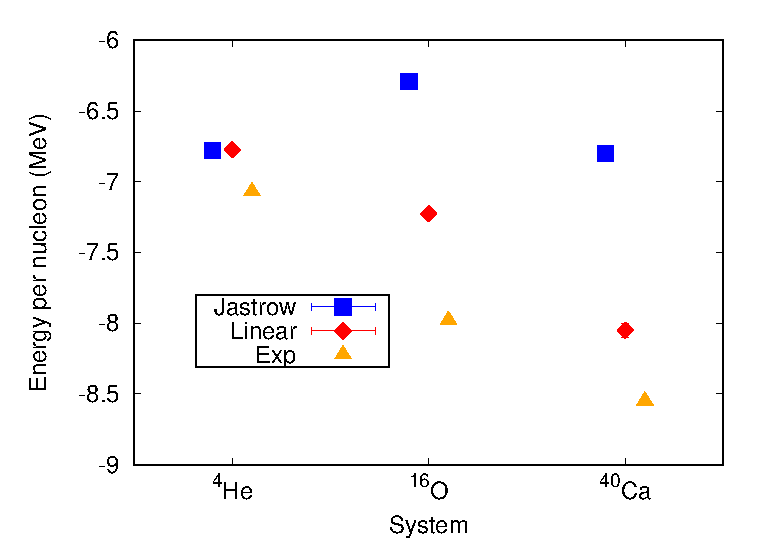
\includegraphics[width=0.7\textwidth]{figures/energy_jaslin.eps}
   \caption{Binding energy calculations done with Jastrow correlations (\cite{gandolfi2007}) compared to Jastrow plus linear spin-isospin dependent correlations (\cite{gandolfi2014}) all compared to experimental results. All calculations were done with AFDMC and the AV6$'$ potential.}
   \label{fig:energy_jaslin}
\end{figure}
In Figure~\ref{fig:energy_jaslin} it is clear to see that the additional spin-isospin correlations are important for both systems larger than $^4$He.

\subsection{Quadratic Correlations}
In this project I have included correlations up to quadratic order which includes up to 4 nucleons being correlated at once. When expanded to quadratic order the symmetrized product wave function, Equation~\ref{equ:prodpsi}, becomes
\begin{equation}
   \begin{split}
      \ket{\psi_T}_\text{quad} = \Bigg[\prod\limits_{i<j}&f_c(r_{ij})\Bigg] \Bigg[1+\fOpij \\
         & + \frac{1}{2}\fOpij\fOqklquad \Bigg] \ket{\phi}.
   \end{split}
   \label{equ:fullquadcorr}
\end{equation}
The subscripts on the sums, which describe which correlations are allowed, can be hard to visualize and so these correlation diagrams are useful.
\begin{figure}[h]
\newcommand\shift{2.0}
\newcommand\vshift{-1.5} %vertical shift
\newcommand\tshift{0.05} %tiny shift
\newcommand\sep{0.75}
   \centering
   \begin{tikzpicture}[>=latex,scale=1.0]
      \draw (-2*\sep,\sep/2.0) node{\large Allowed};
      \draw (-2*\sep,\sep/2.0+\vshift) node{\large Not Allowed};

      \filldraw[black] (0*\shift,0)          circle (2pt) node[anchor=east] {\large j};
      \filldraw[black] (0*\shift,\sep)       circle (2pt) node[anchor=east] {\large i};
      \filldraw[black] (0*\shift+\sep,0)     circle (2pt) node[anchor=west] {\large l};
      \filldraw[black] (0*\shift+\sep,\sep)  circle (2pt) node[anchor=west] {\large k};
      \draw[black, ultra thick] (0*\shift,\sep) -- (0*\shift,0); %i-j
      \draw[black, ultra thick] (0*\shift+\sep,\sep) -- (0*\shift+\sep, 0); %k-l

      \filldraw[black] (1*\shift,0)          circle (2pt) node[anchor=east] {\large k};
      \filldraw[black] (1*\shift,\sep)       circle (2pt) node[anchor=east] {\large i};
      \filldraw[black] (1*\shift+\sep,0)     circle (2pt) node[anchor=west] {\large l};
      \filldraw[black] (1*\shift+\sep,\sep)  circle (2pt) node[anchor=west] {\large j};
      \draw[black, ultra thick] (1*\shift,\sep) -- (1*\shift+\sep,\sep); %i-j
      \draw[black, ultra thick] (1*\shift,0) -- (1*\shift+\sep,0); %k-l

      \filldraw[black] (2*\shift,0)          circle (2pt) node[anchor=east] {\large l};
      \filldraw[black] (2*\shift,\sep)       circle (2pt) node[anchor=east] {\large i};
      \filldraw[black] (2*\shift+\sep,0)     circle (2pt) node[anchor=west] {\large j};
      \filldraw[black] (2*\shift+\sep,\sep)  circle (2pt) node[anchor=west] {\large k};
      \draw[black, ultra thick] (2*\shift,\sep) -- (2*\shift+\sep,0); %i-j
      \draw[black, ultra thick] (2*\shift+\sep,\sep) -- (2*\shift,0); %k-l

      \filldraw[black] (3*\shift,0)          circle (2pt) node[anchor=east] {\large j};
      \filldraw[black] (3*\shift,\sep)       circle (2pt) node[anchor=east] {\large i,k};
      \filldraw[black] (3*\shift+\sep,0)     circle (2pt) node[anchor=west] {\large };
      \filldraw[black] (3*\shift+\sep,\sep)  circle (2pt) node[anchor=west] {\large l};
      \draw[black, ultra thick] (3*\shift,\sep) -- (3*\shift,0); %i-j
      \draw[black, ultra thick] (3*\shift,\sep) -- (3*\shift+\sep,\sep); %k-l

      \filldraw[black] (4*\shift,0)          circle (2pt) node[anchor=east] {\large k};
      \filldraw[black] (4*\shift,\sep)       circle (2pt) node[anchor=east] {\large i};
      \filldraw[black] (4*\shift+\sep,0)     circle (2pt) node[anchor=west] {\large j,l};
      \filldraw[black] (4*\shift+\sep,\sep)  circle (2pt) node[anchor=west] {\large };
      \draw[black, ultra thick] (4*\shift,\sep) -- (4*\shift+\sep,0); %i-j
      \draw[black, ultra thick] (4*\shift,0) -- (4*\shift+\sep,0); %k-l

      \filldraw[black] (2*\shift,\vshift)             circle (2pt) node[anchor=east] {\large j,l};
      \filldraw[black] (2*\shift,\sep+\vshift)        circle (2pt) node[anchor=east] {\large i,k};
      \filldraw[black] (2*\shift+\sep,\vshift)        circle (2pt) node[anchor=west] {\large };
      \filldraw[black] (2*\shift+\sep,\sep+\vshift)   circle (2pt) node[anchor=west] {\large };
      \draw[black, ultra thick] (2*\shift-\tshift,\sep+\vshift) -- (2*\shift-\tshift,\vshift); %i-j
      \draw[black, ultra thick] (2*\shift+\tshift,\sep+\vshift) -- (2*\shift+\tshift,\vshift); %k-l
   \end{tikzpicture}
   \caption{Diagrams used to visualize which correlations are included in the quadratic correlations in Equation~\ref{equ:fullquadcorr}.}
   \label{fig:quaddiagrams}
\end{figure}
All pair correlations are included in this wave function except pairs that are directly correlated with themselves, e.g. $\mathcal{O}_{23}\mathcal{O}_{23}$, where $\mathcal{O}_{ij}$ is a product of single particle operators such as $\si\cdot\sj$ and $\mathcal{O}_{ij}=\mathcal{O}_{ji}$ due to the operators on different particles operating in different Hilbert spaces. For correlations where the same particle is included twice, the correlation operators do not commute and that term must be explicitly symmetrized. Currently in Equation~\ref{equ:fullquadcorr} and in the code all quadratic terms are symmetrized, e.g. the correlation $\mathcal{O}_{12}\mathcal{O}_{34}$ is symmetrized as $\frac{1}{2}\left(\mathcal{O}_{12}\mathcal{O}_{34}+\mathcal{O}_{34}\mathcal{O}_{12}\right)$, even though only terms like $\mathcal{O}_{12}\mathcal{O}_{13}$ need this explicit symmetrization. This adds needless calculation time, but as I'll show, these terms don't seem to be significant and can be omitted completely.

If the exponentially correlated wave function, Equation~\ref{equ:exppsi}, is expanded in the typical way, i.e. $\exp(A) = 1 + A + \frac{1}{2}A^2 + \ldots$, then the quadratic correlations for the exponential wave function become
\begin{equation}
   \begin{split}
      \ket{\psi_T}_\text{exp\_quad} = \Bigg[\prod\limits_{i<j}&f_c(r_{ij})\Bigg] \Bigg[1+\fOpij \\
         & + \frac{1}{2}\fOpij\fOqklexpquad \Bigg] \ket{\phi}.
   \end{split}
   \label{equ:expquadcorr}
\end{equation}
Unlike the quadratic correlations derived from the symmetrized product this wave function includes all of the the terms in Figure~\ref{fig:quaddiagrams}. There is not a large difference between these wave functions up to quadratic order and for here forward all references to quadratic correlations will refer to the expansion from the symmetrized product wave function.

Another way to include quadratic correlations is to only include terms that do not correlate the same particle twice leaving only independent pair correlations. This is the same whether you start from the exponentially correlated or the symmetrized product wave function and it can be written as
\begin{equation}
   \begin{split}
      \ket{\psi_T}_\text{ip} = \Bigg[\prod\limits_{i<j}&f_c(r_{ij})\Bigg] \Bigg[1+\fOpij \\
      & + \fOpij\fOqklip \Bigg] \ket{\phi}
   \end{split}
   \label{equ:ipquadcorr}
\end{equation}
and the independent pair sum can be visualized as in Figure~\ref{fig:ipdiagrams}.
\begin{figure}[h]
\newcommand\shift{2.2}
\newcommand\vshift{-1.5} %vertical shift
\newcommand\tshift{0.05} %tiny shift
\newcommand\sep{0.75}
   \centering
   \begin{tikzpicture}[>=latex,scale=1.0]
      \draw (-3*\sep,\sep/2.0) node{\large Allowed};
      \draw (-3*\sep,\sep/2.0+\vshift) node{\large Not Allowed};

      \filldraw[black] (0*\shift,0)          circle (2pt) node[anchor=east] {\large j};
      \filldraw[black] (0*\shift,\sep)       circle (2pt) node[anchor=east] {\large i};
      \filldraw[black] (0*\shift+\sep,0)     circle (2pt) node[anchor=west] {\large l};
      \filldraw[black] (0*\shift+\sep,\sep)  circle (2pt) node[anchor=west] {\large k};
      \draw[black, ultra thick] (0*\shift,\sep) -- (0*\shift,0); %i-j
      \draw[black, ultra thick] (0*\shift+\sep,\sep) -- (0*\shift+\sep, 0); %k-l

      \filldraw[black] (1*\shift,0)          circle (2pt) node[anchor=east] {\large k};
      \filldraw[black] (1*\shift,\sep)       circle (2pt) node[anchor=east] {\large i};
      \filldraw[black] (1*\shift+\sep,0)     circle (2pt) node[anchor=west] {\large l};
      \filldraw[black] (1*\shift+\sep,\sep)  circle (2pt) node[anchor=west] {\large j};
      \draw[black, ultra thick] (1*\shift,\sep) -- (1*\shift+\sep,\sep); %i-j
      \draw[black, ultra thick] (1*\shift,0) -- (1*\shift+\sep,0); %k-l

      \filldraw[black] (2*\shift,0)          circle (2pt) node[anchor=east] {\large l};
      \filldraw[black] (2*\shift,\sep)       circle (2pt) node[anchor=east] {\large i};
      \filldraw[black] (2*\shift+\sep,0)     circle (2pt) node[anchor=west] {\large j};
      \filldraw[black] (2*\shift+\sep,\sep)  circle (2pt) node[anchor=west] {\large k};
      \draw[black, ultra thick] (2*\shift,\sep) -- (2*\shift+\sep,0); %i-j
      \draw[black, ultra thick] (2*\shift+\sep,\sep) -- (2*\shift,0); %k-l

      \filldraw[black] (0*\shift,\vshift)          circle (2pt) node[anchor=east] {\large j};
      \filldraw[black] (0*\shift,\sep+\vshift)       circle (2pt) node[anchor=east] {\large i,k};
      \filldraw[black] (0*\shift+\sep,\vshift)     circle (2pt) node[anchor=west] {\large };
      \filldraw[black] (0*\shift+\sep,\sep+\vshift)  circle (2pt) node[anchor=west] {\large l};
      \draw[black, ultra thick] (0*\shift,\sep+\vshift) -- (0*\shift,\vshift); %i-j
      \draw[black, ultra thick] (0*\shift,\sep+\vshift) -- (0*\shift+\sep,\sep+\vshift); %k-l

      \filldraw[black] (1*\shift,\vshift)          circle (2pt) node[anchor=east] {\large k};
      \filldraw[black] (1*\shift,\sep+\vshift)       circle (2pt) node[anchor=east] {\large i};
      \filldraw[black] (1*\shift+\sep,\vshift)     circle (2pt) node[anchor=west] {\large j,l};
      \filldraw[black] (1*\shift+\sep,+\vshift)  circle (2pt) node[anchor=west] {\large };
      \draw[black, ultra thick] (1*\shift,\sep+\vshift) -- (1*\shift+\sep,\vshift); %i-j
      \draw[black, ultra thick] (1*\shift,\vshift) -- (1*\shift+\sep,\vshift); %k-l

      \filldraw[black] (2*\shift,\vshift)             circle (2pt) node[anchor=east] {\large j,l};
      \filldraw[black] (2*\shift,\sep+\vshift)        circle (2pt) node[anchor=east] {\large i,k};
      \filldraw[black] (2*\shift+\sep,\vshift)        circle (2pt) node[anchor=west] {\large };
      \filldraw[black] (2*\shift+\sep,\sep+\vshift)   circle (2pt) node[anchor=west] {\large };
      \draw[black, ultra thick] (2*\shift-\tshift,\sep+\vshift) -- (2*\shift-\tshift,\vshift); %i-j
      \draw[black, ultra thick] (2*\shift+\tshift,\sep+\vshift) -- (2*\shift+\tshift,\vshift); %k-l
   \end{tikzpicture}
   \caption{Diagrams used to visualize which correlations are included in the independent pair quadratic correlations in Equation~\ref{equ:ipquadcorr}.}
   \label{fig:ipdiagrams}
\end{figure}
All terms where a particle is included twice in the correlation are ignored, as a results, all correlation operators commute and the correlations are explicitly symmetric. Neither of these correlations maintain the strong condition of cluster decomposability. Like the linear correlations, each product of states does not contain all of the needed correlations, though these wave functions contain more than the linear correlations. An effort to build an antisymmetric and cluster decomposable wave function from the exponentially correlated wave function will be discussed later.

The energy and it's uncertainty are often used to judge the convergence of a propagated wave function in QMC and so a good wave function needs to be able to reproduce known binding energies. To this end I have calculated binding energies with the linear, quadratic, and independent pair (IP) quadratic correlations derived from the symmetrized product for $^4$He, $^{16}$O, $^{40}$Ca, and symmetric nuclear matter (SNM) at saturation density, $\rho_0=0.16$ fm$^{-3}$, in a period box with 28 particles. The trial states for SNM are built from plane waves and 7 particles fills the first plane wave shell. This is why we have done calculations with 28 particles, 7 for each of the spin-isospin states. The energy per particle for nuclei is plotted in Figure~\ref{fig:energies} and the specific energies can be found in Table~\ref{tab:energies}.
\begin{figure}[h!]
   \centering
   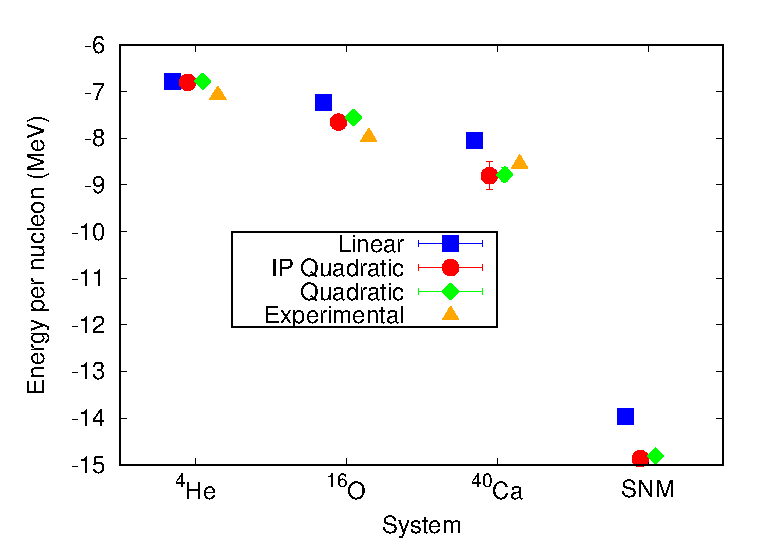
\includegraphics[width=0.7\textwidth]{figures/energy.eps}
   \caption{Energy per particle for small and medium closed shell nuclei with no Coulomb interaction calculated with the AFDMC method with the AV6$'$ interaction. Each calculations was done with the linear, IP quadratic, and quadratic correlations. Energies are compared to experimental values where available and the statistical uncertainties are included. The variational parameters were reoptimized for each wave function the $^4$He calculations, however the $^{16}$O, $^{40}$Ca, and SNM calculations were done starting with VMC trial wave functions with linear correlations.}
   \label{fig:energies}
\end{figure}
\begin{table}[htb]
   \centering
   \begin{tabular}{ccccc}
      \hline\hline
      System & Linear & Ind-Pair & Quadratic & Experimental \\
      \hline
      $^4${He}    & -6.785(10)   & -6.798(8) & -6.778(8)    & -7.074 \\   
      $^{16}${O}  & -7.23(6)     & -7.65(9)  & -7.55(8)     & -7.98  \\   
      $^{40}${Ca} & -8.05(8)     & -8.8(3)   & -8.78(15)    & -8.55  \\
      SNM         & -13.97(3)    & -14.87(4) & -14.70(11)   &        \\
      \hline\hline
   \end{tabular}
   \caption{Energy per particle from AFDMC calculations with no Coulomb interaction with the AV6$'$ interaction. Each calculations was done with the linear, independent pair, and quadratic correlations. Energies are compared to experimental values where available and the statistical uncertainties are included.}
   \label{tab:energies}
\end{table}
All calculations were done with trial wave functions coming from VMC calculations with linear correlations, except for $^4$He, which was performed by reoptimizing the variational parameters for each set of correlations. This was done due to the complexity of optimizing the parameters for large systems. Like with the addition of Jastrow correlations in Figure~\ref{fig:energy_jaslin}, all systems larger than $^4$He decreased in energy with additional correlations, while the binding energy for $^4$He was the same to within uncertainties. In addition, the energies for all systems are identical to within uncertainties for the quadratic and IP quadratic correlations, indicating that the IP correlations capture most of the relevant physics. As a result any further references to quadratic correlations will be referring to the IP quadratic correlations, as these correlations are computationally less expensive, unless a distinction is made otherwise. The percent decrease in energy for $^{16}$O and $^{40}$Ca when adding linear correlations is 15\% and 18\% respectively. When adding quadratic correlations the energies decrease an additional 6\% and 9\% respectively. This indicates that each successive term in the expansion decreases in importance. It is important to note that these calculations were done with the AV6$'$ potential, which is a limited 2-nucleon potential. We do not expect our energies to be equal to experiment due to the lack of the full 2-body, and a complete lack of the 3-body force. The AV6$'$ potential has been used to simplify the calculations and to look for qualitative improvements caused by the additional correlations. Some calculations have been done using more sophisticated potentials with the quadratic correlations, and those results will be shown later.

The energies above are calculated with the AFDMC method. As mentioned before, the fixed phase approximation is used to solve the Fermi sign problem within AFDMC, and as such the energies are not constrained by the upper bounds to the ground state energy, as evidenced by the results for $^{40}$Ca, which is actually overbound. The lack of an upper bound prevents us to say strictly that the decrease in energy is because of an improvement in the trial wave function. However, all calculations were first done with the VMC method, which does provide an upper bound constraint. As can be seen in Figure~\ref{fig:energies_vmc} and Table~\ref{tab:energies_vmc}, the same conclusions found with the AFDMC calculations are also found with the VMC calculations, as we can say that the quadratic wave functions are actually an improvement. As mentioned before, releasing the constraint can sometimes give convergence to the true energy, or at least give an indication of the direction to the true ground state energy.

\begin{figure}[h!]
   \centering
   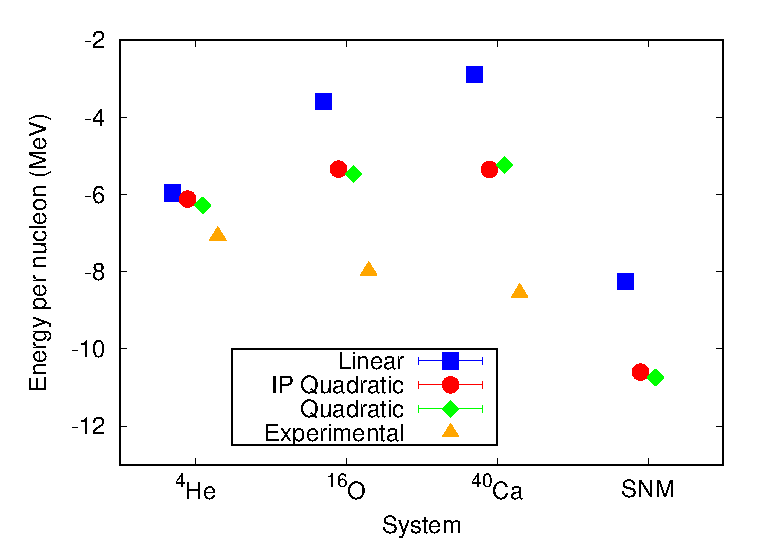
\includegraphics[width=0.7\textwidth]{figures/energy_vmc.eps}
   \caption{Energy per particle for small and medium closed shell nuclei with no Coulomb interaction calculated with the VMC method with the AV6$'$ interaction. Each calculations was done with the linear, independent pair, and quadratic correlations. Energies are compared to experimental values where available and the statistical uncertainties are included. Unlike the above results, calculated with the AFDMC method, these VMC results are an upper bound to the ground state energy.}
   \label{fig:energies_vmc}
\end{figure}
\begin{table}[htb]
   \centering
   \begin{tabular}{ccccc}
      \hline\hline
      System & Linear & Ind-Pair & Quadratic & Experimental \\
      \hline
      $^4${He}    & -5.955(10)   & -6.113(8) & -6.275(5)    & -7.074 \\   
      $^{16}${O}  & -3.581(3)    & -5.338(3) & -5.463(3)    & -7.98  \\   
      $^{40}${Ca} & -2.88(5)     & -5.35(5)  & -5.23(5)     & -8.55  \\
      SNM         & -8.25(4)     & -10.60(3) & -10.74(2)    &        \\
      \hline\hline
   \end{tabular}
   \caption{Energy per particle from VMC calculations with no Coulomb interaction with the AV6$'$ interaction. Unlike the AFDMC results, these VMC results provide an upper bound to the energy. Each calculations was done with the linear, independent pair, and quadratic correlations. Energies are compared to experimental values where available and the statistical uncertainties are included.}
   \label{tab:energies_vmc}
\end{table}

There is a significant decrease in energy with the addition of the quadratic correlations, however, there is an additional cost to calculating these additional terms. I have calculated a scaling factor, which is the ratio of times taken to calculate a given block of code, including the propagation of walkers spatial and spin components as well as the calculation of the energies, for linear compared to linear plus quadratic correlations. A scaling factor of 2 would mean that the calculation took twice as long with the quadratic correlations as it did without. The scaling factors are plotted in Figure~\ref{fig:scaling} and the specific values are in Table~\ref{tab:scaling}.
\begin{figure}[h!]
   \centering
   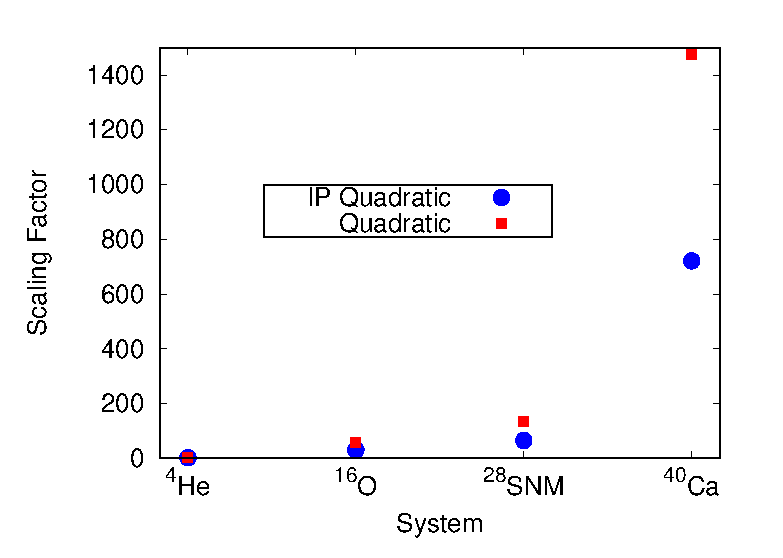
\includegraphics[width=0.7\textwidth]{figures/scaling.eps}
   \caption{Scaling factors calculated as the ratio of times taken to calculate a given block of code for linear and linear plus quadratic correlations.}
   \label{fig:scaling}
\end{figure}
\begin{table}[htb]
   \centering
   \begin{tabular}{ccccc}
      \hline \hline
       & $^{4}$He & $^{16}$O & SNM(28) & $^{40}$Ca \\
      \hline
      IP Quadratic & 1.73 & 30.7 & 64.8 & 720.9 \\
      Quadratic & 2.00 & 58.8 & 133.6 & 1473.9 \\
      \hline \hline
   \end{tabular}
   \caption{Same scaling factors that are calculated in Figure~\ref{fig:scaling}.}
   \label{tab:scaling}
\end{table}
The scaling for the quadratic correlations is about twice that of the IP quadratic correlations. This is due to the explicit symmetrization that is done for each quadratic term in the quadratic correlations. This could be decreased if commuting terms were not symmetrized, however as noted before the IP quadratic correlations seem to capture the important physics, and so all future calculations with quadratic correlations will be using the IP correlations. The IP correlations all commute and so no explicit symmetrization is needed. A typical AFDMC calculation using only linear correlations for $^{16}$O with 1000 walkers takes on the order of a tens of CPU hours and a similar calculation for $^{40}$Ca takes on the order of hundreds of CPU hours.

The number of quadratic terms in the IP correlations given $A$ particles is
\begin{equation}
   N_\text{ip}=\frac{A(A-1)(A-2)(A-3)}{8}.
\end{equation}
For the fully quadratic wave function the number of terms given $A$ particles is
\begin{equation}
   N_\text{quad}=\frac{A(A-1)}{2}\left(\frac{A(A-1)}{2}-1\right),
\end{equation}
where $A(A-1)/2$ is the number of possible pairs made from $A$ particles. If the fully quadratic correlations are not explicitly symmetrized for the IP terms then this reduces to $N_\text{quad}-N_\text{ip}$. In Figure~\ref{fig:scaling_theory} I have plotted the number of terms for the independent pair, fully quadratic, and fully quadratic correlations without symmetrizing the IP terms.
\begin{figure}[h!]
   \centering
   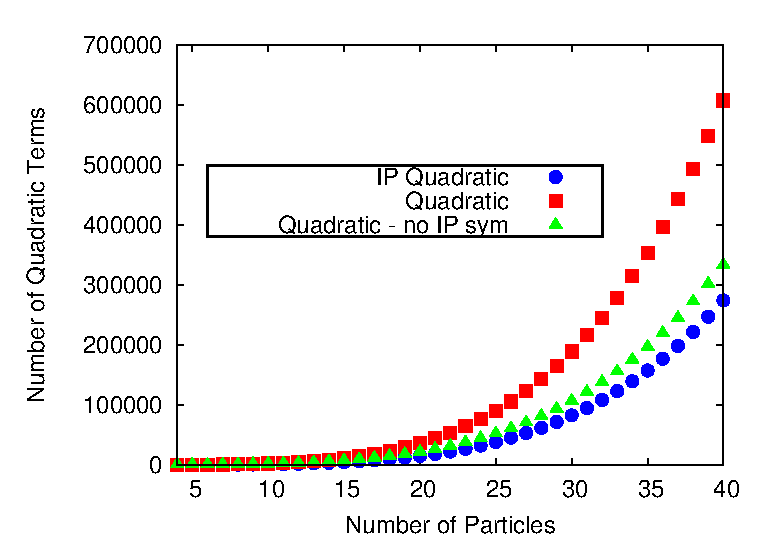
\includegraphics[width=0.7\textwidth]{figures/scaling_theory.eps}
   \caption{Number of terms in the quadratic correlations for the IP, quadratic, and quadratic correlations without explicit symmetrization of the IP terms.}
   \label{fig:scaling_theory}
\end{figure}

In recent years efforts have been made to fit infinite matter saturation properties with microscopic nuclear interactions (\cite{drischler2017}). Calculations of energies near saturation using AFDMC have not been able to fit known saturation properties. I have done calculations of symmetric nuclear matter near saturation with and without quadratic correlations, using only the AV6$'$ 2-body interaction and have compared these results to known saturation properties in Figure~\ref{fig:saturation}. Though 3N forces will surely be needed to obtain a good fit, it is clear that improved correlations are also going to be needed.
\begin{figure}[h!]
   \centering
   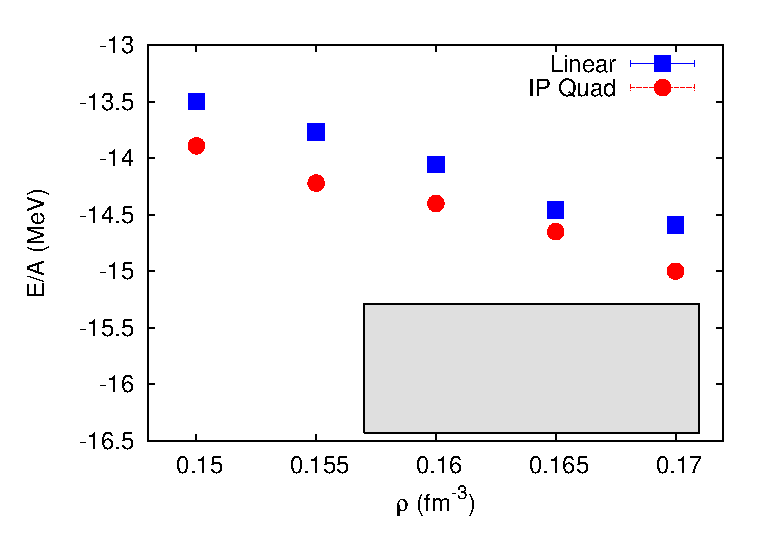
\includegraphics[width=0.7\textwidth]{figures/saturation.eps}
   \caption{Energy calculations done using the AV6$'$ potential with linear and quadratic correlations. The gray box is the same empirical saturation region used in \cite{drischler2017}, $\rho_0 = 0.164 \pm 0.007$ fm$^{-3}$ and $E/A=-15.86 \pm 0.57$ MeV.}
   \label{fig:saturation}
\end{figure}

\subsection{Calculating the Two-Body Operators}
When calculating expectation values with the additional two-body operators of the quadratic correlations, the scaling will increase from $O(A^4)$ to $O(A^6)$ for the calculation of the energy and from $O(A^2)$ to $O(A^4)$ for the calculation of the trial wave function alone. This can be quite expensive, especially for large systems. As a result we have used a technique to reduce the number of calculations by performing recurring pieces of the calculations only once at the beginning. Though this doesn't decrease the polynomial scaling it does decrease the factor in front of the polynomial scaling.

The Slater Determinant is the base ingredient to calculating the trial wave function. The Slater matrix is defined as
\begin{equation}
   S = \begin{pmatrix}
      \braket{\alpha_1}{\r_1,s_1} & \braket{\alpha_1}{\r_2,s_2} & \ldots & \braket{\alpha_1}{\r_A,s_A} \\
      \braket{\alpha_2}{\r_1,s_1} & \braket{\alpha_2}{\r_2,s_2} & \ldots & \braket{\alpha_2}{\r_A,s_A} \\
      \vdots & \vdots & \ddots & \vdots \\
      \braket{\alpha_A}{\r_1,s_1} & \braket{\alpha_A}{\r_2,s_2} & \ldots & \braket{\alpha_A}{\r_A,s_A}
   \end{pmatrix},
\end{equation}
where each matrix element will be written as
\begin{equation}
   S_{\alpha i} = \braket{\alpha}{\r_i,s_i}.
\end{equation}
This can be written in terms of the spin-isospin basis as
\begin{equation}
   S_{\alpha i} = \sum\limits_{\gamma=1}^4 \braket{\alpha}{\r_i \chi_\gamma}\braket{\chi_\gamma}{s_i}.
\end{equation}
where $\r_i$ and $s_i$ are the positions and spin-isospin configurations of the system, and $\ket{\alpha}$ contains the radial part of the wave function and the spherical harmonics that give the proper angular momentum to each state. The $\ket{\chi_\gamma}$ basis is given in terms of $\ket{p\uparrow}$, $\ket{p\downarrow}$, $\ket{n\uparrow}$, and $\ket{n\downarrow}$ as
\begin{equation}
\begin{split}
   \ket{\chi_1} &= \ket{\left(1,0,0,0\right)} \\
   \ket{\chi_2} &= \ket{\left(0,1,0,0\right)} \\
   \ket{\chi_3} &= \ket{\left(0,0,1,0\right)} \\
   \ket{\chi_4} &= \ket{\left(0,0,0,1\right)}.
\end{split}
\end{equation}

The Slater matrix is updated once for every single-body operator and twice for every two-body operator using the identity
\begin{equation}
   \det{\left(S^{-1}S'\right)} = \frac{\det{S'}}{\det S},
   \label{equ:matrixid}
\end{equation}
where $S'$ is the Slater matrix that has been updated due to the operation of a single-body operator.

Using the identity in Equation~\ref{equ:matrixid} allows us to calculate the product $S^{-1}S''$, where $S''$ represents the Slater matrix with only the $i$ and $j$ columns updated. The product $S^{-1}S$ would give the identity matrix and so $S^{-1}S''$ is the identity matrix everywhere except for the columns $i$ and $j$
\begin{equation}
   S^{-1}S'' = 
   \begin{pmatrix}
      1 & 0 & \ldots & \bra{\alpha_1}\mathcal{O}_i\ket{\r_i,s_i} & \ldots & \bra{\alpha_1}\mathcal{O}_j\ket{\r_j,s_j} & \ldots & 0 & 0 \\
      0 & 1 & \ldots & \bra{\alpha_2}\mathcal{O}_i\ket{\r_i,s_i} & \ldots & \bra{\alpha_2}\mathcal{O}_j\ket{\r_j,s_j} & \ldots & 0 & 0 \\
      \vdots & \vdots & \ddots & \vdots & \ddots & \vdots & \ddots & \vdots & \vdots \\
      0 & 0 & \ldots & \bra{\alpha_A}\mathcal{O}_i\ket{\r_i,s_i} & \ldots & \bra{\alpha_A}\mathcal{O}_j\ket{\r_j,s_j} & \ldots & 0 & 1 \\
   \end{pmatrix}.
\end{equation}
The determinant is then equal to the determinant of the submatrix given by keeping only the elements $\left(S^{-1}S''\right)_{mn}$ where $m$ and $n$ are both of the changed columns
\begin{equation}
   \det{S^{-1}S''} =
   \det\begin{pmatrix}
      \bra{\alpha_i}\mathcal{O}_i\ket{\r_i,s_i} & \bra{\alpha_i}\mathcal{O}_j\ket{\r_j,s_j} \\
      \bra{\alpha_j}\mathcal{O}_i\ket{\r_i,s_i} & \bra{\alpha_j}\mathcal{O}_j\ket{\r_j,s_j} \\
   \end{pmatrix}.
\end{equation}

In practice the calculation of a two-body operator $\mathcal{O}_{ij}=\mathcal{O}_i\mathcal{O}_j$ is calculated as
\begin{equation}
   \frac{\bra{\Phi}\mathcal{O}_{ij}\ket{RS}}{\braket{\Phi}{RS}} = \sum\limits_{\gamma=1}^4\sum\limits_{\delta=1}^4 d_{2b}(\chi_\gamma,\chi_\delta,ij)\bra{\chi_\gamma\chi_\delta}\mathcal{O}_{ij}\ket{s_is_j},
   \label{equ:d2bdef}
\end{equation}
where $R=\{\r_1,\ldots,\r_A\}$ and $S=\{s_1,\ldots,s_A\}$ are the spatial and spin-isospin configurations and
\begin{equation}
   d_{2b}(\chi_\gamma,\chi_\delta,ij)=\frac{\langle\Phi|R,s_1,\ldots,s_{i-1},\chi_\gamma,s_{i+1},\ldots,s_{j-1},\chi_\delta,s_{j+1},\ldots,s_A\rangle}{\langle \Phi|RS\rangle}.
\end{equation}
Note that as part of the update the basis states $\chi_\gamma$ and $\chi_\delta$ have replaced the spin-isospin configurations $s_i$ and $s_j$ respectively.

To reduce the number of calculations done in the inner loops of the calculation the matrix $P_{\chi,ij}$ is defined and precalculated as
\begin{align}
   P_{\chi_\gamma,ij} &=\sum_\alpha S^{-1}_{j\alpha}S_{\alpha i}(s_i\leftarrow \chi_\gamma), \\
   P_{\chi_\delta,ij} &=\sum_\alpha S^{\prime\;-1}_{j\alpha}S^\prime_{\alpha i}(s_j\leftarrow \chi_\delta).
\end{align}
The $d_{2b}$ distribution can then be written as
\begin{equation}
   d_{2b}(\chi_\gamma,\chi_\delta,ij)=\det\begin{pmatrix}P_{\chi_\gamma,ii} & P_{\chi_\gamma,ij} \\ P_{\chi_\delta,ji} & P_{\chi_\delta,jj}\end{pmatrix},
\end{equation}
and thus the $d_{2b}$ can be precalculated and multiplied by each operator expectation value $\bra{\chi_\gamma\chi_\delta}\mathcal{O}_{ij}\ket{s_is_j}$ from Equation~\ref{equ:d2bdef}.

This description has been for 2-body operators, however the quadratic operators involve 4-body operators for the correlations of the trial wave function, and 6-body operators for the calculations of the energy. This method can also be extended to $n$-body operators by updating the $P$ matrix to use the previously updated Slater matrices
\begin{equation}
   P_{\chi_\eta,mn}=\sum_\alpha S^{\prime\prime\;-1}_{n\alpha}S^{\prime\prime}_{\alpha m}(s_m\leftarrow \chi_\eta),
\end{equation}
where each iteratively updated matrix $S'$ is calculated from the last $S$ as
\begin{align}
   S^{\prime}_{\alpha m}(s_m) = \left\{
   \begin{array}{cc}
      S_{\alpha m} & m \ne i\\
      \langle\alpha|\mathcal O_i|\mathbf{r}_i\,s_i\rangle  & m = i
   \end{array} .
   \right.
\end{align}
The updated inverse matrix is calculated by again using the identity in Equation~\ref{equ:matrixid}, expanding both sides and grouping like terms, noting that $S''_{mi} = S'_{mi}$ when $j\ne i$. The next iteration of the updated inverse matrix $S'^{-1}$ is calculated as
\begin{equation}
S'^{-1}_{jn} = \left \{
\begin{array}{cc}
S^{-1}_{jn} -\frac{\sum_m S^{-1}_{jm}S'_{mi}}{\sum_\ell S^{-1}_{i\ell}
S'_{\ell i}} S^{-1}_{in}  & j \ne i\\
\frac{S^{-1}_{in}}{\sum_m S^{-1}_{im}S'_{mi}} & j = i\\
\end{array}
\right . \,.
\end{equation}

To calculate the wave function in Equation~\ref{equ:linearcorr} with only linear correlations the correlation operators are first acted on the spin-isospin basis states which are then summed together with the $d_{2b}$ as
\begin{equation}
   \sum\limits_{\chi_\gamma,\chi_\delta}d_{2b}(\chi_\gamma,\chi_\delta,ij)\langle\chi_\gamma,\chi_\delta|f_{ij}^p\mathcal{O}_{ij}^p|s_i s_j\rangle.
\end{equation}
The potential introduces two additional operators and so the expectation value of the potential with the linear wave function is calculated as $(\mathbb{1}+\mathcal{O}^c_{ij})\mathcal{O}^p_{kl}$ where $\mathcal{O}^c$ and $\mathcal{O}^p$ are the correlation and potential operators respectively and can be four distinct operators. This calculation is done by first updating the $P$ matrix twice, once for each of $\mathcal{O}^c_i$ and $\mathcal{O}^c_j$ where $\mathcal{O}_{ij}=\mathcal{O}_i\mathcal{O}_j$. The determinant in Equation~\ref{equ:d2bdef} is then calculated using the updated $d''_{2b}$.

Both versions of the quadratic correlations in Equations~\ref{equ:fullquadcorr} and \ref{equ:ipquadcorr} have the form $\mathbb{1} + \mathcal{O}^c_{ij} + \mathcal{O}^c_{ij}\mathcal{O}^c_{kl}$. The first is exactly the linear correlations and are calculated in the same way as described above. The quadratic operators looks like the potential operator with linear correlations with $\mathcal{O}^c_{ij}\mathcal{O}^p_{kl} \rightarrow \mathcal{O}^c_{ij}\mathcal{O}^c_{kl}$ and so the same method can be followed as described before by updating the $P$ matrix twice. The number of operations required for the linear correlations scales as $O(A^2)$ while the quadratic correlations, as well as the expectation value of the potential with linear correlations, scales as $O(A^4)$.

The expectation value of the potential as calculated with the quadratic correlations takes the form $\left(\mathbb{1} + \mathcal{O}^c_{ij} + \mathcal{O}^c_{ij}\mathcal{O}_{kl}^c\right)\mathcal{O}^p_{mn}$. The only piece that is not similar to previous descriptions is the $\mathcal{O}^c_{ij}\mathcal{O}^c_{kl}\mathcal{O}^p_{mn}$ piece. This can be calculated by using four distinct updates of the $P$ matrix, one for each of the four correlations operators. The updates are first done for the $\mathcal{O}^c_{ij}$ operators after which two additional updates are performed for the $\mathcal{O}^c_{kl}$ operators. This is used to calculate the expectation value of the $\mathcal{O}^p_{mn}$ operators. The scaling to calculate the expectation value of the potential with quadratic correlations is $O(A^6)$.

Additional details about the quadratic correlations and how the operator updates are performed can be found in our recent paper \cite{lonardoni2018}.

\subsection{Quadratic Correlations with NN and 3N $\chi$EFT Potentials}
The results presented above have been done with the simplified AV6$'$ NN potential. This choice was made to reduce the computational cost of testing the improved correlations. The new quadratic correlations have also been used with more sophisticated potentials, namely, those developed in the $\chi$EFT framework. We have done preliminary calculations with the $\chi$EFT potential up to N$^2$LO in the chiral expansion. Higher orders of the chiral expansion are still inaccessible to QMC calculations due to their non-locality. We have obtained preliminary results (Diego Lonardoni, private communication, 2019) of binding energy calculations for $^4$He, $^{16}$O, and SNM with 28 particles in a periodic box at saturation density. Both the VMC and AFDMC preliminary results are shown in Table~\ref{tab:chiquad}.
\begin{table}[htb]
   \centering
   \begin{tabular}{llccc}
      \hline
      Calculation & Correlations & $^4$He & $^{16}$O & SNM \\
      \hline
      VMC   & Linear       & $-5.86(1)$ & $-1.08(1)$ & $1.56(5)$ \\
      VMC   & IP Quadratic & $-$        & $-4.03(4)$ & $-$ \\
      VMC   & Quadratic    & $-6.72(1)$ & $-3.95(4)$ & $-$ \\
      \hline
      AFDMC & Linear       & $-6.89(2)$ & $-5.74(4)$ & $-9.5(1)$ \\
      AFDMC & IP Quadratic & $-$        & $-7.3(2)$  & $-12.5(1)$ \\
      AFDMC & Quadratic    & $-6.91(2)$ & $-6.9(2)$  & $-12.6(1)$ \\
      \hline
   \end{tabular}
   \caption{Ground state energies of $^4$He, $^{16}$O, and SNM with 28 particles at saturation density, calculated with the VMC and AFDMC methods. All energies are reported as energy/nucleon in MeV. The trial wave functions are calculated with both 2- and 3-body correlations, where all three 2-body correlations were used. For all calculations the N$^2$LO local chiral potential with the $R_0 = 1$ fm cutoff as described in our paper (\cite{lonardoni2018}). Additional details about each calculation are given in the text. Not all possible calculations were performed, and dashes are places where data does not exist.}
   \label{tab:chiquad}
\end{table}
All calculations were done with 2- and 3-body correlations, however the 2-body correlations were varied to include the linear, IP quadratic, and the fully quadratic correlations. The potential used in these calculations was the local chiral potential expanded to N$^2$LO with a cutoff of $R_0=1$ fm. The $^4$He and SNM calculations were done with the $E\mathbb{1}$ parameterization, while the $^{16}$O calculations were done with the $E\tau$ parameterization as described in our paper \cite{lonardoni2018}. The $^4$He and $^{16}$O calculations included the coulomb force and were reoptimized for each set of correlations. Due to the computational cost of reoptimizing the variational parameters with the quadratic wave functions the AFDMC calculations for SNM were done using the trial wave function obtained from a VMC calculations with linear correlations. In addition the AFDMC calculations for SNM were done using the growth energy, which is a diagnostic tool which is similar to the local energy for small time steps. If the trial wave function was exactly the ground state and the offset energy $E_0$ the exact ground state energy, then the weights of the walkers would all be 1, regardless of the configuration. This leads to the definition of the growth energy
\begin{equation}
\left<E_G\right> = E_0-\frac{1}{\Delta\tau}\log{(\left<w\right>)}.
\end{equation}
More details on the growth energy are given in \cite{lynn2013}. All AFDMC calculation were performed with the constrained-path approximation. The 2-body operator structure of the N$^2$LO chiral interaction is the same as the AV7$'$ potential which adds the spin-orbit $\mathbf{L}\cdot\mathbf{S}$ term to the AV6$'$ interaction. It was shown in \cite{gandolfi2014} that the AV7$'$ potential provides less binding than the AV6$'$ potential for the systems shown here. This explains why the energies are slightly higher here than with the AV6$'$ results shown in the preceding sections. However, the decrease in energy between the linear and quadratic correlations is much larger when the 3-body interactions are included. The decrease in the $^{16}$O energy between linear correlations and IP quadratic correlations with only the AV6$'$ NN potential was 6\%, while the same system had a decrease of 27\% with the NN+3N N$^2$LO potential. This was expected as we expected the additional correlations to have a larger overlap with the 3-body force than the original linear correlations.

\subsection{Exponential Correlations}
From the wave function using the expansion up to quadratic terms it is clear that an improved trial wave function is necessary to describe the state of larger nuclei and nuclear matter. It was also shown in the previous sections that expanding the current wave functions described in Equations~\ref{equ:exppsi} and \ref{equ:prodpsi}, is not an efficient method to improve the wave function, as the cost of each additional term grows exponentially. However, another option is to evaluate the full wave function using a Monte Carlo sampling. The exponential wave function is written as
\begin{equation}
   \ket{\Psi_T} = \left[\prod\limits_{i<j}f_c(r_{ij})\right] e^{\sum\limits_{i<j,p}f_p(r_{ij})\Oijp} \ket{\Phi},
\end{equation}
which has the same operator form as the spin-isospin propagator used in AFDMC, where again, the operators are the AV6$'$ operators, $\si\cdot\sj$, $\ti\cdot\tj$, $\si\cdot\sj \ti\cdot\tj$, $S_{ij}$ and $S_{ij} \ti\cdot\tj$, where $S_{ij} = 3\si\cdot\hat{r}_{ij}\sj\cdot\hat{r}_{ij}-\si\cdot\sj$. These operators are written in terms of squared single particle operators, allowing for the Hubbard Stratanovich transformation to express the correlations in terms of a single particle operator and integrals over auxiliary fields, which are evaluated via Monte Carlo.

The correlation functions $f_p(r_{ij})$ are written in terms of symmetric matrices
\begin{equation}
\begin{split}
   \exp\left(\sum\limits_{i<j,p}f_p(r_{ij})\Oijp\right) = \exp&\left(\frac{1}{2}\sum\limits_{i\alpha,j\beta} \sigma_{i\alpha}A^{\sigma}_{i\alpha,j\beta}\sigma_{j\beta}\right. \\
      &\left. + \frac{1}{2}\sum\limits_{i\alpha,j\beta} \sigma_{i\alpha}A^{\sigma\tau}_{i\alpha,j\beta}\sigma_{j\beta}\ti\cdot\tj
      + \frac{1}{2}\sum\limits_{i,j} A^{\tau}_{i,j}\ti\cdot\tj\right),
   \label{equ:amatrices}
\end{split}
\end{equation}
which can be written in terms of their eigenvalues and eigenvectors
\begin{align}
   &\sum\limits_{j\beta} A^{\sigma}_{i\alpha,j\beta}\psi^{\sigma}_{n,j\beta} = \lambda^{\sigma}_n\psi^{\sigma}_{n,i\alpha} \\
   &\sum\limits_{j\beta} A^{\sigma\tau}_{i\alpha,j\beta}\psi^{\sigma\tau}_{n,j\beta} = \lambda^{\sigma\tau}_n\psi^{\sigma\tau}_{n,i\alpha} \\
   &\sum\limits_{j} A^{\tau}_{i,j}\psi^{\tau}_{n,j} = \lambda^{\tau}_n\psi^{\tau}_{n,i}.
\end{align}
The correlations are then written in terms of squared single particle operators,
\begin{equation}
\begin{split}
   \exp\left(\sum\limits_{i<j,p}f_p(r_{ij})\Oijp\right) = \exp&\left(\frac{1}{2}\sum\limits_{n=1}^{3A} \left(O_{n}^{\sigma}\right)^2 \lambda_n^{\sigma}\right. \\
      & \left. + \frac{1}{2}\sum\limits_{\gamma=1}^{3}\sum\limits_{n=1}^{3A} \left(O_{n\gamma}^{\sigma\tau}\right)^2 \lambda_n^{\sigma\tau}
      + \frac{1}{2}\sum\limits_{\gamma=1}^{3}\sum\limits_{n=1}^{A} \left(O_{n\gamma}^{\tau}\right)^2 \lambda_n^{\tau}\right),
\end{split}
\end{equation}
where the operators are given by
\begin{equation}
\begin{split}
   O_{n}^{\sigma} &= \sum\limits_{i\alpha} \sigma_{i\alpha}\psi_{n,i\alpha}^{\sigma} \\
   O_{n\gamma}^{\sigma\tau} &= \sum\limits_{i\alpha} \tau_{i\gamma}\sigma_{i\alpha}\psi_{n,i\alpha}^{\sigma\tau} \\
   O_{n\gamma}^{\tau} &= \sum\limits_{i} \tau_{i\gamma}\psi_{n,i}^{\tau}.
   \label{equ:OA}
\end{split}
\end{equation}
This can be written in a more compact form,
\begin{equation}
    \exp\left(\sum\limits_{i<j,p}f_p(r_{ij})\Oijp\right) = \exp\left(\frac{1}{2}\sum\limits_{n=1}^{15A} \left(O_{n}\right)^2 \lambda_n^{\sigma}\right).
\end{equation}
The Hubbard Stratanovich transformation is then used to write these as single particle operators and integrals over auxiliary fields, $x_n$. Ignoring commutator terms this can be written as
\begin{equation}
   \exp\left(\frac{1}{2}\sum\limits_{n=1}^{15A} \left(O_{n}\right)^2 \lambda_n^{\sigma}\right) = \prod\limits_{n=1}^{15A} \frac{1}{\sqrt{2\pi}}\int dx_n e^{-x_n^2/2}e^{\sqrt{\lambda_n}x_nO_n}.
\end{equation}

The auxiliary fields are then drawn from the Gaussian distribution, $\exp\left(-x_n^2/2\right)$ and the correlations can be written as
\begin{equation}
   \Psi_T(R,S) = \bra{RS}\prod\limits_{n=1}^{15A} \frac{1}{N} \sum\limits_{\{x_n\}}^N\frac{1}{\sqrt{2\pi}}e^{\sqrt{\lambda_n}x_nO_n}\ket{\Phi}.
\end{equation}
The $\{x_n\}$ are the set of 15$A$ auxiliary fields, one for each of the different 15$A$ operators.

Large errors arise with this first naive approach. This is due to the ordering of the eigenvectors as given by the algorithm. When derivatives of the wave function are taken the eigenvectors may be given in a different order for each term in the numerical derivative, and thus each vector could be paired with a different random sample of the auxiliary fields. One approach to remove this issue is to use a product of square roots of the $A$ matrices.

This can be done by rewriting Equation~\ref{equ:amatrices} as
\begin{equation}
\begin{split}
   \exp\left(\sum\limits_{i<j,p}f_p(r_{ij})\Oijp\right) = \exp&\left(\frac{1}{2}\sum\limits_{i\alpha,j\beta} \sigma_{i\alpha}\sum\limits_{k\gamma}\left(A^{\sigma}_{i\alpha,k\gamma}\right)^{1/2}\left(A^{\sigma}_{k\gamma,j\beta}\right)^{1/2}\sigma_{j\beta}\right. \\
      & + \frac{1}{2}\sum\limits_{i\alpha,j\beta} \sigma_{i\alpha}\sum\limits_{k\gamma}\left(A^{\sigma\tau}_{i\alpha,k\gamma}\right)^{1/2}\left(A^{\sigma\tau}_{k\gamma,j\beta}\right)^{1/2}\sigma_{j\beta}\ti\cdot\tj \\
      &\left. + \frac{1}{2}\sum\limits_{i,j} \sum\limits_{k}\left(A^{\tau}_{i,k}\right)^{1/2}\left(A^{\tau}_{k,j}\right)^{1/2}\ti\cdot\tj\right),
\end{split}
\end{equation}
where we have rewritten the matrices using the definition $A_{a,b} = \sum_cA^{1/2}_{a,c}A^{1/2}_{c,b}$. These square root matrices can be written, similar to before, in terms of their eigenvalues and vectors as
\begin{align}
   &\sum\limits_{j\beta} \left(A^{\sigma}_{i\alpha,j\beta}\right)^{1/2}\psi^{\sigma}_{n,j\beta} = \left(\lambda^{\sigma}_n\right)^{1/2}\psi^{\sigma}_{n,i\alpha} \\
   &\sum\limits_{j\beta} \left(A^{\sigma\tau}_{i\alpha,j\beta}\right)^{1/2}\psi^{\sigma\tau}_{n,j\beta} = \left(\lambda^{\sigma\tau}_n\right)^{1/2}\psi^{\sigma\tau}_{n,i\alpha} \\
   &\sum\limits_{j} \left(A^{\tau}_{i,j}\right)^{1/2}\psi^{\tau}_{n,j} = \left(\lambda^{\tau}_n\right)^{1/2}\psi^{\tau}_{n,i}.
\end{align}
As before, this can be used to rewrite the correlations in terms of squared single particle operators
\begin{equation}
\begin{split}
   \exp\left(\sum\limits_{i<j,p}f_p(r_{ij})\Oijp\right) = \exp&\left(\frac{1}{2}\sum\limits_{k\delta=1}^{3A} \left(O_{k\delta}^{\sigma}\right)^2\right. \\
      & \left. + \frac{1}{2}\sum\limits_{\gamma=1}^{3}\sum\limits_{k\delta=1}^{3A} \left(O_{k\delta,\gamma}^{\sigma\tau}\right)^2
      + \frac{1}{2}\sum\limits_{\gamma=1}^{3}\sum\limits_{k=1}^{A} \left(O_{k,\gamma}^{\tau}\right)^2\right).
\end{split}
\end{equation}
where the operators are now
\begin{equation}
\begin{split}
   O_{k\delta}^{\sigma} &= \sum\limits_{i\alpha}\sum\limits_n \sigma_{i\alpha}\psi_{n,i\alpha}^\sigma\left(\lambda_n^\sigma\right)^{1/2}\psi_{n,k\delta}^{\sigma} \\
   O_{k\delta,\gamma}^{\sigma\tau} &= \sum\limits_{i\alpha}\sum\limits_n \tau_{i\gamma}\sigma_{i\alpha}\psi_{n,i\alpha}^{\sigma\tau}\left(\lambda_n^{\sigma\tau}\right)^{1/2}\psi_{n,k\delta}^{\sigma\tau} \\
   O_{k\delta}^{\tau} &= \sum\limits_{i}\sum\limits_n \tau_{i\gamma}\psi_{n,i}^\tau\left(\lambda_n^\tau\right)^{1/2}\psi_{n,k}^{\tau}.
\end{split}
\end{equation}
I have combined the sums over $k=1,\ldots,A$ and $\delta=1,2,3$ into a single sum $k\delta=1,\ldots,3A$.

The difference between these operators and those described in Equation~\ref{equ:OA} is the explicit sum over the eigenvector ordering, as given by the label $n$. Like before each of these operators will be coupled with a sampled auxiliary field, however the operators maintain their order regardless of the ordering of the eigenvectors. This removes any systematic errors from the ordering of the eigenvectors. More details on this derivation can be found in Appendix~\ref{app:a12}.

Minimal success has been achieved with these correlations for light nuclei (\cite{bouadani2009_dissertation}), however there are large uncertainties that make this wave function currently infeasible to use. Removing these uncertainties could make this wave function a very useful tool for nuclear QMC as it can be systematically improved by increasing the number of samples of the auxiliary fields.

Another possibility for decreasing statistical error is to use the plus-minus sampling technique as described in Section~\ref{sec:AFDMC}. Because the auxiliary fields are sampled from a Gaussian centered at zero, the probability of a given sample $x_n$ is the same as the probability for the sample $-x_n$. As a result, the wave function for both samples can be calculated and the sample with the larger weight can be accepted. Additional work needs to be made before this wave function is implemented in production. However, the scaling of this wave function is better for large systems compared to that of the quadratic correlations, and so this wave function may, in the future, be more suitable for calculations of larger systems. Also, systematic improvements can be made to the trial wave function by including additional samples of the auxiliary fields, or by explicitly evaluating some correlations as in the linear and quadratically correlated wave functions.

%\subsection{Alessandro's correlations and $T^2$ fix to them}
%\red{Maybe just do $T^2$ fix and apply it to exponential correlations \ldots maybe don't include this at all.}
